\documentclass{beamer}
\usepackage{amsmath,amsbsy,amsopn,amstext,amsfonts,amssymb}
\usepackage{isomath}
\usepackage{ulem}
%\linespread{1.6}  % double spaces lines
\usepackage{graphicx}
\usepackage{subfigure}
\usepackage{color}
\usepackage{optidef}  % define optimization problems
\usepackage{multicol}  % multiple columns
\usepackage{listings} % for python code
\usepackage{mathrsfs}

\usepackage{polynom}
\newcommand{\adj}{\mathrm{adj}}
\newcommand{\constrainedmin}[3]{
		\begin{mini*}|s|
		{#2}{#1}{}{}
		\addConstraint{#3}
		\end{mini*}
}

\newcommand{\rwbcomment}[1]{{\color{blue}RWB:#1}}
\newcommand{\defeq}{\stackrel{\triangle}{=}}
\newcommand{\abs}[1]{\left|#1\right|}
\newcommand{\norm}[1]{\left\|#1\right\|}
\newcommand{\iprod}[1]{\left<#1\right>}
\newcommand{\ellbf}{\boldsymbol{\ell}}
\newcommand{\nubf}{\boldsymbol{\nu}}
\newcommand{\mubf}{\boldsymbol{\mu}}
\newcommand{\abf}{\mathbf{a}}
\newcommand{\bbf}{\mathbf{b}}
\newcommand{\cbf}{\mathbf{c}}
\newcommand{\dbf}{\mathbf{d}}
\newcommand{\ebf}{\mathbf{e}}
\newcommand{\fbf}{\mathbf{f}}
\newcommand{\gbf}{\mathbf{g}}
\newcommand{\hbf}{\mathbf{h}}
\newcommand{\ibf}{\mathbf{i}}
\newcommand{\jbf}{\mathbf{j}}
\newcommand{\kbf}{\mathbf{k}}
\newcommand{\lbf}{\mathbf{l}}
\newcommand{\mbf}{\mathbf{m}}
\newcommand{\nbf}{\mathbf{n}}
\newcommand{\obf}{\mathbf{o}}
\newcommand{\pbf}{\mathbf{p}}
\newcommand{\qbf}{\mathbf{q}}
\newcommand{\rbf}{\mathbf{r}}
\newcommand{\sbf}{\mathbf{s}}
\newcommand{\tbf}{\mathbf{t}}
\newcommand{\ubf}{\mathbf{u}}
\newcommand{\vbf}{\mathbf{v}}
\newcommand{\wbf}{\mathbf{w}}
\newcommand{\xbf}{\mathbf{x}}
\newcommand{\ybf}{\mathbf{y}}
\newcommand{\zbf}{\mathbf{z}}
\newcommand{\Jbf}{\mathbf{J}}
\newcommand{\Acal}{\mathcal{A}}
\newcommand{\Bcal}{\mathcal{B}}
\newcommand{\Lcal}{\mathcal{L}}
\newcommand{\Ncal}{\mathcal{N}}
\newcommand{\Rcal}{\mathcal{R}}
\definecolor{darkolivegreen}{rgb}{0.33, 0.42, 0.18}

\makeatletter
\newenvironment<>{proofstart}[1][\proofname]{%
    \par
    \def\insertproofname{#1\@addpunct{.}}%
    \usebeamertemplate{proof begin}#2}
  {\usebeamertemplate{proof end}}
\newenvironment<>{proofcont}{%
  \setbeamertemplate{proof begin}{\begin{block}{}}
    \par
    \usebeamertemplate{proof begin}}
  {\usebeamertemplate{proof end}}
\newenvironment<>{proofend}{%
    \par
    \pushQED{\qed}
    \setbeamertemplate{proof begin}{\begin{block}{}}
    \usebeamertemplate{proof begin}}
  {\popQED\usebeamertemplate{proof end}}
\makeatother

\title{ECEn 671: Mathematics of Signals and Systems \\ 
Moon: Chapter 14.}
\author{Randal W. Beard}
\institute{Brigham Young University}
\date{\today}

\begin{document}

%-------------------------------
\begin{frame}
	\titlepage
\end{frame}

%-------------------------------
\begin{frame}[t]
\frametitle{Table of Contents}
\tableofcontents
\end{frame}

%%%%%%%%%%%%%%%%%%%%%%%%%%%%%%%%%%%%%%%%%%%%%%%%%%%%%%%%%%%%%%%%%
\section{Gradient Descent}
\frame{\sectionpage}


%----------------------------------
\begin{frame}\frametitle{Gradient Descent}
	The topic for the remainder of the course is minimization and maximization of functions.
	
	\vfill
	
	In particular we will constrain our attention to continuously differentiable functions.
\end{frame}

%----------------------------------
\begin{frame}\frametitle{Gradient Descent}
	Suppose we have a function of the form
	\begin{center}
		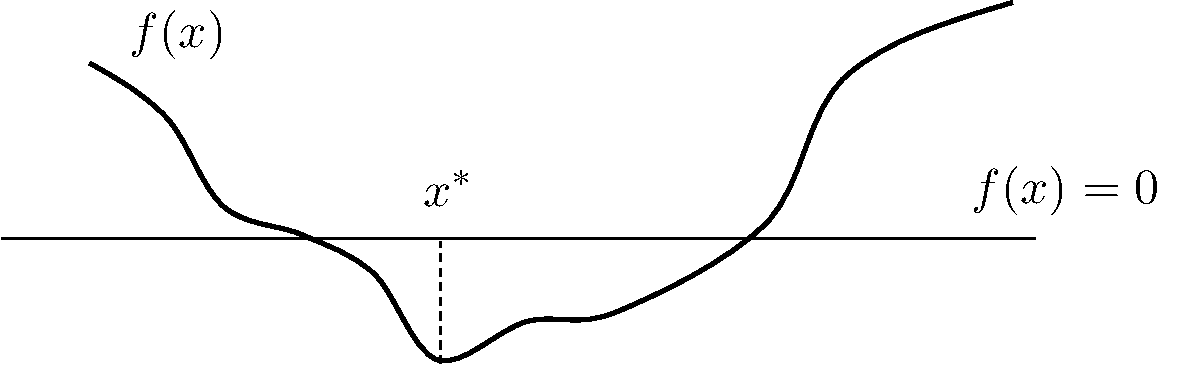
\includegraphics[width=0.5\textwidth]
			{figures/chap14_function_with_minimum}
	\end{center}
	and we would like to find $x^{\ast}$, what should we do?
\end{frame}

%----------------------------------
\begin{frame}\frametitle{Gradient Descent}
	The basic idea of gradient descent is to pick any $x^{[0]}$ and then move ``downward''.  To move down, we look at the slope of $f$.
	
	\vfill
	
	If $\frac{\partial f}{\partial x}(x^{[k]})$ is positive, chose $x^{[k+1]} < x^{[k]}$.
	
	\vfill
	
	If $\frac{\partial f}{\partial x}(x^{[k]})$ is negative, choose $x^{[k+1]} > x^{[k]}$
	
	\vfill
	
	i.e.
	\[ 
		x^{[k+1]} = x^{[k]} - \alpha \frac{\partial f}{\partial x}(x^{[k]}),
	\]
	where $\alpha$ is the step size.	
\end{frame}

%----------------------------------
\begin{frame}\frametitle{Gradient Descent}
	Before moving to the multivariable case, lets consider the potential problems with this approach.	
	
	\vfill
	
	{\color{blue}Problem 1: Local Minima.}
	If $f$ looks like this:
	\begin{center}
		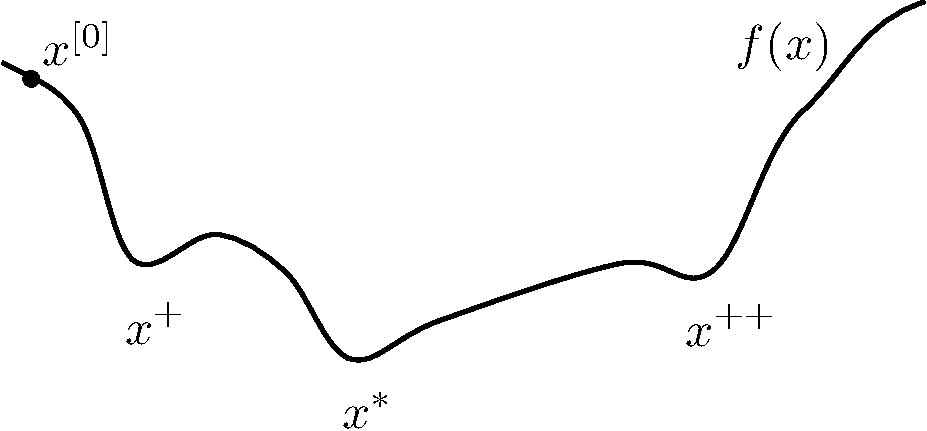
\includegraphics[width=0.5\textwidth]
			{figures/chap14_function_gradiant_descent}
	\end{center}
	then if the initial condition is at $x^{[0]}$, the iteration 
	\[
		x^{[k+1]} = x^{[k]} - \alpha \frac{\partial f}{\partial x}(x^{[k]})
	\] 
	will converge to $x^+$, if $\alpha$ is small enough.
\end{frame}

%----------------------------------
\begin{frame}\frametitle{Gradient Descent}
	Other initial conditions will result in 
	$x^{++}$ while others will give $x^\ast$, the true minimum.
	
	\vfill
	
	This is a fundamental problem with \underline{any} method that relies on derivative information.  There are no completely satisfactory solutions to the problem.  However there are many ad-hoc fixes.	

	\vfill
	
	\begin{example}
		\begin{itemize}
		\item Execute from numerous ``random'' initial conditions and pick the lowest solution.
		\item Occassionally introduce random jumps in $x$.
		\item etc...
		\end{itemize}
	\end{example}
\end{frame}

%----------------------------------
\begin{frame}\frametitle{Gradient Descent}
	{\color{blue}Problem 2: Step Size.}
	The selection of $\alpha$ can have a major effect on the convergence of the sequence
	\[ 
		x^{[k+1]} = x^{[k]} - \alpha \frac{\partial f}{\partial x}(x^{[k]}) 
	\]
	
	For example,
	\begin{center}
		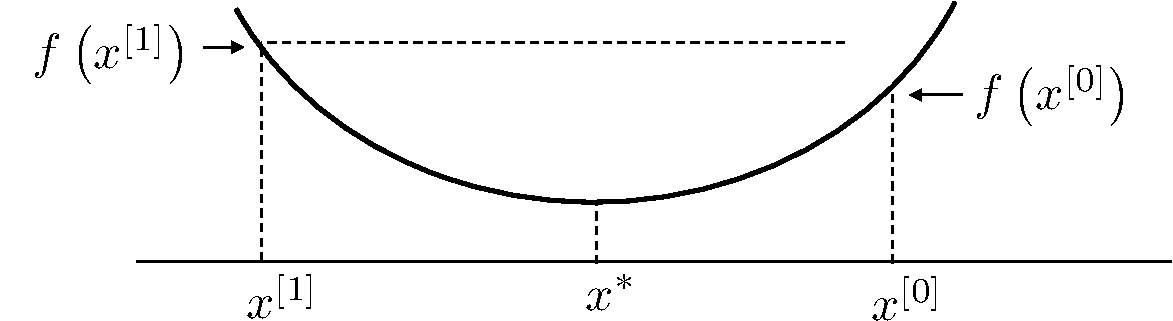
\includegraphics[width=0.5\textwidth]
			{figures/chap14_quadratic}
	\end{center}
	Note $f$ is very steep on sides, so $\alpha \frac{\partial f}{\partial x}(x^{[k]})$ could be large.  This could cause $x^{[1]}$ to overshoot the minimum.  This could cause (1) instability, (2) limit cycles, (3) extremely slow and oscillatory convergence	
\end{frame}

%----------------------------------
\begin{frame}\frametitle{Gradient Descent}

	{\color{blue}Lesson:}  
		Don't make $\alpha$ too large.
		
	\vfill
	
	However if $\alpha$ is too small, then convergence will be very slow.
	
	\vfill
	
	Most implementations adapt the size of $\alpha$.
\end{frame}

%%%%%%%%%%%%%%%%%%%%%%%%%%%%%%%%%%%%%%%%%%%%%%%%%%%%%%%%%%%%%%%%%
\section{Gradient Descent: Multivariable Case}
\frame{\sectionpage}

%----------------------------------
\begin{frame}\frametitle{Gradient Descent: Multivariable Case}
	Let $f:\mathbb{R}^n\to\mathbb{R}$ be a multivariable function.
	\begin{example}
		If $x \in \mathbb{R}^n$ then 
		$f(x) = x_1^2 + x_2^2 + \cdots + x_n^2$ maps $\mathbb{R}^n\to\mathbb{R}$.	
	\end{example}
	The gradient of a multivariable function is
	\[ 
		\frac{\partial  f}{\partial  x} = \begin{pmatrix}
	    \frac{\partial  f}{\partial  x_1}\\
	    \vdots\\
	    \frac{\partial  f}{\partial  x_n}
	  \end{pmatrix} 
	\] 
	and maps $\mathbb{R}^n \to \mathbb{R}^n$.
\end{frame}

%----------------------------------
\begin{frame}\frametitle{Gradient Descent: Multivariable Case}
	\begin{example}
		If $f(x) = x_1^2 + \cdots + x_n^2$ then
		\( 
			\frac{\partial  f}{\partial  x} 
				= \begin{pmatrix}
		    		2x_1\\
		    		2x_2\\
		    		\vdots\\
		    		2x_n
		  		  \end{pmatrix}
		\)		
	\end{example}

	\begin{center}
		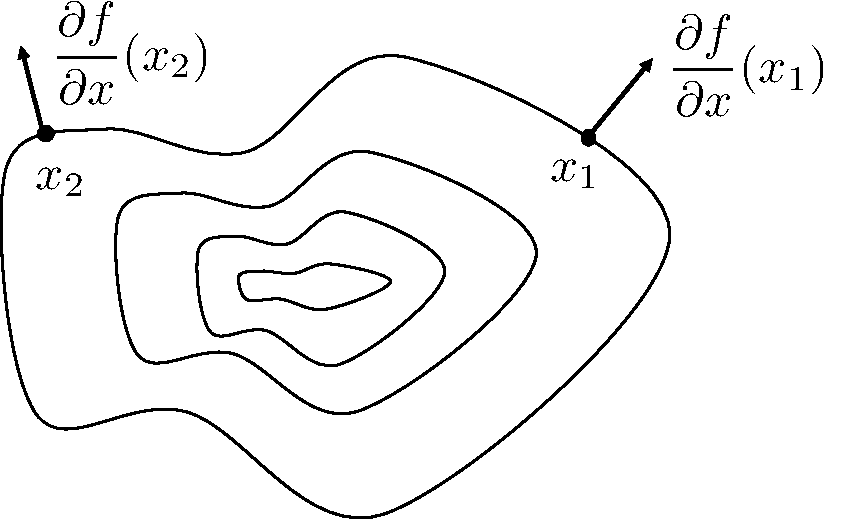
\includegraphics[width=0.5\textwidth]
			{figures/chap14_2D_gradiant}
	\end{center}
	The gradient points perpendicular to the level curves of $f$.	
\end{frame}

%----------------------------------
\begin{frame}\frametitle{Gradient Descent: Multivariable Case}
	\begin{theorem}[Moon Theorem 14.5]
		Let $f:\mathbb{R}^m \to \mathbb{R}$ be a differentiable function in some open set $D$.  The gradient $\frac{\partial  f}{\partial  x}(x)$ points in the direction of the maximum increase of $f$ at the point $x$.		
	\end{theorem}
\end{frame}

%----------------------------------
\begin{frame}\frametitle{Gradient Descent: Multivariable Case}
	\begin{proof}
		Expand $f(x+\lambda y)$ in a Taylor series as
		\[ 
			f(x + \lambda y) = f(x) + \lambda\frac{\partial  f^T}{\partial  x}(x)y + \text{Higher Order Terms (HOT)} 
		\]
		where HOT. are $O(\lambda^2)$, i.e.,
		\[
			\lim_{\lambda \to 0}\frac{H.O.T.}{\lambda} = 0.
		\]	
		We would like to find $y$ that maximizes $f(x + \lambda y)$ as $\lambda \to 0$.

		By Cauchy-Schwartz, $\frac{\partial  f^T}{\partial  x}y$ is maximized when $y = \frac{\partial  f}{\partial  x}$.	
	\end{proof}
\end{frame}

%----------------------------------
\begin{frame}\frametitle{Gradient Descent: Multivariable Case}
	For multivarible functions, the gradient descent formula is
	\[ 
		\fbox{$x^{[k+1]} = x^{[k]} - \alpha_k \frac{\partial f}{\partial x}(x^{[k]})$}
	\]
	
	Again, the selection of the step size is very important.  If $\alpha_k$ is too small convergence will be slow.
	
	\vfill
	
	If $\alpha_k$ is too large, algorithm could be unstable.	
	
	\vfill
	
	How to pick the right $\alpha$?
	
\end{frame}

%----------------------------------
\begin{frame}\frametitle{Gradient Descent: Multivariable Case}
	Locally around a min or max, every smooth function can be approximated by a quadratic (Taylor series).  
	
	\vfill
	
	We can gain insight about the selection of $\alpha$ by studying quadratic functions.
	
	\vfill
	
	Let $f(x) = x^TRx - 2b^Tx$ where $x \in \mathbb{R}^m,b\in\mathbb{R}^m,R=R^T>0$.	
	
	\vfill
	
	Taking the gradient we get
	\[ 
		\frac{\partial f}{\partial x} = 2Rx - 2b.
	\]
\end{frame}

%----------------------------------
\begin{frame}\frametitle{Gradient Descent: Multivariable Case}
	So the gradient descent algorithm is
	\[ 
		x^{[k+1]} = x^{[k]} - 2\alpha(Rx^{[k]} - b). 
	\]
	Let $x^{\ast}$ satisfy $Rx^{\ast}=b$ then
	\[ 
		x^{[k+1]} - x^{\ast} = x^{[k]} - x^{\ast} - 2\alpha(Rx^{[k]} - Rx^{\ast}) 
	\]
	Define $y^{[k]} = x^{[k]} - x^{\ast}$ and $\mu = 2\alpha$, then 
	\begin{align*}
		y^{[k+1]} 
			&= y^{[k]} - \mu R y^{[k]} \\
			&= (I - \mu R)y^{[k]}\\
		\implies y^{[k]} &= (I - \mu R)^ky^{[0]}.
	\end{align*}	
\end{frame}

%----------------------------------
\begin{frame}\frametitle{Gradient Descent: Multivariable Case}
	Since $R$ is symmetric positive definite
	\[ 
		R = Q\Lambda Q^T 
	\]
	where $Q$-orthogonal.
	Therefore,
	\begin{align*}
		y^{[k]} 
			&= (QQ^T-\mu Q\Lambda Q^T)^ky^{[0]}\\
			&= Q(I-\mu\Lambda)^kQ^Ty^{[0]}
	\end{align*}
	Letting $z = Q^Ty$,
	\begin{align}
		& z^{[k]} = (I - \mu\Lambda)^kz^{[0]}\\
		\implies &
		z^{[k]}_i = (1 - \mu \lambda_i)^kz_i^{[0]}
	\end{align}
	which converges if $\abs{1-\mu\lambda_i} < 1$, $i = 1, \ldots, m$.	
\end{frame}

%----------------------------------
\begin{frame}\frametitle{Gradient Descent: Multivariable Case}
	Therefore, convergence happens when
	\begin{align*}
	-1 &< 1 - \mu \lambda_i < 1 \\
	\iff -2 &< -\mu\lambda_i < 0\\
	\iff 0 &< \mu\lambda_i < 2\\
	\iff 0 &< \mu < \frac{2}{\lambda_i} 
	\end{align*}
	Recall that $\lambda_i > 0$ when $R$ is positive definite, 
	so if
	\[ 
		0 < \alpha < \frac{1}{\lambda_{\max}(R)} 
	\]
	then steepest descent converges for quadratic functions.
\end{frame}

%----------------------------------
\begin{frame}\frametitle{Gradient Descent: Multivariable Case}
	Note that the convergence along each eigenaxis is determined by 
	\(
		\frac{1}{\lambda_i}.
	\)	
	
	\vfill

	Therefore if $R$ is ill-conditioned, i.e., $\displaystyle \frac{\lambda_{\max}}{\lambda_{\min}}$ is large, then convergence for gradient descent will be much slower along some axes than others.	
\end{frame}

%%%%%%%%%%%%%%%%%%%%%%%%%%%%%%%%%%%%%%%%%%%%%%%%%%%%%%%%%%%%%%%%%
\section{Application:  LMS Adaptive Filtering}
\frame{\sectionpage}

%----------------------------------
\begin{frame}\frametitle{LMS Adaptive Filtering}
		
	\begin{center}
		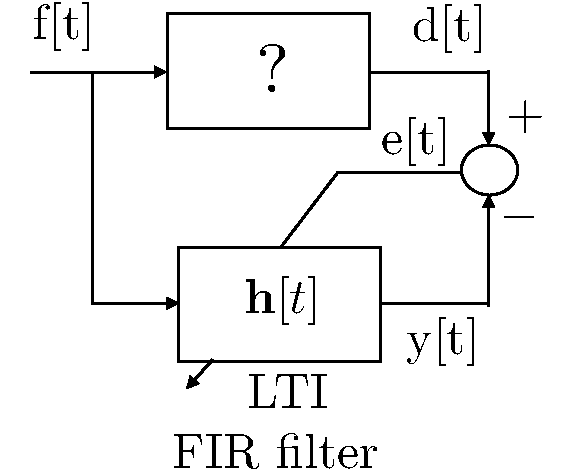
\includegraphics[width=0.5\textwidth]
			{figures/chap14_adaptive_filter}
	\end{center}
	Recall the RLS adaptive filter algorithm.
	
	The objective is to minimize the error
	\[ 
		J(\hbf) = (d[t] - y[t])^2.
	\]
	
	\begin{itemize}
		\item The RLS minimizes the squared error of all past outputs, but LMS only minimizes the squared error of the current output.
		\item The RLS algorithm was derived using the projection theorem.
		\item LMS is derived using gradient descent.
	\end{itemize}
\end{frame}

%----------------------------------
\begin{frame}\frametitle{LMS Adaptive Filtering}
	Assume that the output of the adaptive filter is
	\[ 
		y[t] = \sum_{\ell = 0}^{m-1}h[\ell]f[t-\ell] = \fbf^\top[t]\hbf
	\]
	where
	\[
		\fbf[t] 
			= \begin{pmatrix}
	    		f[t]\\
	    		f[t-1]\\
	    		\vdots\\
	    		f[t-m+1]
	  		  \end{pmatrix}
	  	\text{ and }
		\hbf
			= \begin{pmatrix}
	    		h[0]\\
	    		h[1]\\
	    		\vdots\\
	    		h[m-1]
	  		  \end{pmatrix}
	\]
\end{frame}

%----------------------------------
\begin{frame}\frametitle{LMS Adaptive Filtering}
	Then
	\begin{align*}
		J(\hbf) 
			&= (d[t] - y[t])^2 \\
			&= (d[t] - \fbf^\top[t]\hbf)^2\\
			&= d^2[t] - d[t]\fbf^\top[t]\hbf - d[t]\hbf^\top f[t] + \hbf\fbf[t]\fbf^\top[t]\hbf
	\end{align*}
	where 
	\[ 
		\frac{\partial J}{\partial \hbf} 
			= 2\fbf[t]\fbf^\top[t] \hbf - 2d[t]\fbf[t] 
	\]
\end{frame}

%----------------------------------
\begin{frame}\frametitle{LMS Adaptive Filtering}
	So let
	\[ 
		\hbf[t+1] = \hbf[t] - \alpha \frac{\partial J}{\partial \hbf}(\hbf[t]) 
	\]
	gives
	\begin{align*}
		 \hbf[t+1] 
		 	&= \hbf[t] - 2\alpha(\fbf[t]\fbf^\top[t]\hbf[t] - d[t]\fbf[t])\\
			&= \hbf[t] + \mu \fbf[t](d[t] - \fbf^\top[t]\hbf[t])\\
	\end{align*}
	\[
		\fbox{$\hbf[t+1] = \hbf[t] + \mu \fbf[t]e[t]$}
	\]
	This is known as the LMS adaptive filter.
	
	\vfill
	
	Compare to RLS...
	
	For discussion on convergence, consult Moon Chap~14...
\end{frame}

%%----------------------------------
%\begin{frame}\frametitle{LMS Adaptive Filtering}
%	{\color{blue}Question:} Does the LMS algorithm converge?
%	
%	\vfill
%	
%	Since $J(\hbf)$ is quadratic, we suspect it might converge when
%	\[ 
%		0 < \mu < \frac{2}{\lambda_{\max(R)}}. 
%	\]
%	This is shown in the book under some bad assumptions.	
%	Since we don't know $R$ we can proceed as follows:
%	
%	\[ 
%		tr(R) = \sum_{j=1}^m\lambda_j 
%	\]
%	so
%	\[ 
%		\lambda_{\max(R)} \leq \sum_{j=1}^m\lambda_j  \qquad (\lambda_j > 0) 
%	\]
%\end{frame}
%
%%----------------------------------
%\begin{frame}\frametitle{LMS Adaptive Filtering}
%	But
%	\begin{align*}
%		R 
%			&= E\{f[t]f^T[t]\}\\
%			&= E\left\{ 
%					\begin{pmatrix}
%			       		f[t]\\
%			       		f[t-1]\\
%			       		\vdots\\
%			       		f[t-m+1]
%			      	\end{pmatrix}
%			      	\begin{pmatrix}
%			    		f[t] & \cdots & f[t-m+1]
%			  		\end{pmatrix} 
%		  		\right\}\\
%			&= E\left\{ 
%		      		\begin{pmatrix}
%		       			f[t]f[t]\\
%		       			& f[t-1]f[t-1]\\
%		       			& & \ddots\\
%		       			& & & f[t-m+1]f[t-m+1]
%		      		\end{pmatrix}
%				\right\}
%	\end{align*}
%	
%	If $f$ is a random variable with variance $\sigma^2$ then $tr(R) = m\sigma^2$ so if 
%	\[
%		0 < \mu < \frac{2}{m\sigma^2} < \frac{2}{m\lambda_{\max(R)}}
%	\]
%	then LMS converges.	
%\end{frame}

%%%%%%%%%%%%%%%%%%%%%%%%%%%%%%%%%%%%%%%%%%%%%%%%%%%%%%%%%%%%%%%%%
\section{Gauss-Newton Optimization}
\frame{\sectionpage}

%----------------------------------
\begin{frame}\frametitle{Least Squares as a Gradient Descent Problem}
Consider the least squares problem
	\begin{mini*}|s|
		{x\in\mathbb{R}^n}{\norm{Ax-b}_2^2}{}{}
	\end{mini*}
where $A\in\mathbb{R}^{m\times n}$ is tall.  We know that the solution is
\[
x^\ast = (A^\top A)^{-1} A^\top b.
\]

Can we pose this as a gradient descent problem?
\end{frame}

%----------------------------------
\begin{frame}\frametitle{Least Squares as a Gradient Descent Problem}
	Define the \underline{residual} as
	\[
		\rbf(x) = \begin{pmatrix} r_1(x) \\ \vdots \\ r_m(x) \end{pmatrix} = Ax-b
	\]	
	and define the sum-of-squares error as
	\begin{align*}
	S(x) &= \frac{1}{2}\rbf^\top(x)\rbf(x) \\
		 &= \frac{1}{2}\sum_{j=1}^m r_j^2(x) \\
		 &= \frac{1}{2}(Ax-b)^\top (Ax-b) \\
		 &= \frac{1}{2}\norm{Ax-b}_2^2.
	\end{align*}
	The least squares problem is to find $x$ that minimizes $S(x)$.
\end{frame}

%----------------------------------
\begin{frame}\frametitle{Least Squares as a Gradient Descent Problem}
	The gradient of $S$ is given by
	\begin{align*}
		\frac{\partial S}{\partial x} 
			&= \frac{\partial \rbf}{\partial x}^\top(x) \rbf(x) \\
			&= A^\top (Ax-b) = A^\top A x - A^\top b.
	\end{align*}
	
	So the gradient descent algorithm gives
	\[
	x^{[k+1]} = x^{[k]} - \alpha \left(A^\top A x^{[k]} - A^\top b\right)
	\]
	
	In general, we might allow $\alpha>0$ to be a positive definite matrix $\mathscr{A}>0$:
	\[
	x^{[k+1]} = x^{[k]} - \mathscr{A} \left(A^\top A x^{[k]} - A^\top b\right).
	\]	
	
\end{frame}

%----------------------------------
\begin{frame}\frametitle{Least Squares as a Gradient Descent Problem}
	Selecting 
	\[
		\mathscr{A} = (A^\top A)^{-1}
	\]	
	gives
	\begin{align*}
	x^{[k+1]} 
		&= x^{[k]} - (A^\top A)^{-1} \left(A^\top A x^{[k]} - A^\top b\right) \\
		&= x^{[k]} - (A^\top A)^{-1} (A^\top A) x^{[k]} + (A^\top A)^{-1} A^\top b \\
		&= (A^\top A)^{-1} A^\top b,
	\end{align*}
	which is the optimal solution.  
	
	Noting that $A = \frac{\partial \rbf}{\partial x}$, we have shown that the iteration
	\[
	x^{[k+1]} = x^{[k]} - \left(\frac{\partial \rbf^\top}{\partial x}(x^{[k]}) \frac{\partial \rbf}{\partial x}(x^{[k]})\right)^{-1} \frac{\partial \rbf^\top}{\partial x}(x^{[k]}) \rbf(x^{[k]})
	\]
	converges to the optimal in {\em one} step when $\rbf(x) = Ax-b$.
\end{frame}

%----------------------------------
\begin{frame}\frametitle{Nonlinear Least Squares}
	Let $r_j(x)$, $j=1, \dots, m$ be a general set of residual function to be minimized.  In other words, suppose we wish to solve
	\begin{mini*}|s|
		{x\in\mathbb{R}^n}{\frac{1}{2}\rbf^\top(x) \rbf(x)}{}{}.
	\end{mini*}
	Let $\Jbf(x) \defeq \frac{\partial \rbf}{\partial x}(x)$.  Then the \underline{Gauss-Newton} (GN) iteration algorithm is given by
	\[
		x^{[k+1]} = x^{[k]} - \left(\Jbf^\top(x^{[k]}) \Jbf(x^{[k]})\right)^{-1} \Jbf^\top(x^{[k]}) \rbf(x^{[k]})
	\]
	
	We know that the GN method converges in one step for the linear least squares problem.
\end{frame}

%%%%%%%%%%%%%%%%%%%%%%%%%%%%%%%%%%%%%%%%%%%%%%%%%%%%%%%%%%%%%%%%%
\section{Levenberg-Marquardt Optimization}
\frame{\sectionpage}

%----------------------------------
\begin{frame}\frametitle{Nonlinear Least Squares}
	The downside of GN is that the matrix $J^\top(x) J(x)$ may be ill-conditions at some states $x$.
	
	For the general nonlinear least squares problem, we have
	\[
	\frac{\partial \frac{1}{2}\rbf^\top(x) \rbf(x)}{\partial x} = \frac{\partial \rbf^\top}{\partial x}(x) \rbf(x) = \Jbf^\top(x)\rbf(x).
	\]
	Therefore we have
	\begin{align*}
		\text{Gradient Descent} &\quad 	x^{[k+1]} = x^{[k]} - \alpha \Jbf^\top(x^{[k]}) \rbf(x^{[k]}) \\
		\text{Gauss-Newton} &\quad 	x^{[k+1]} = x^{[k]} - \left(\Jbf^\top(x^{[k]}) \Jbf(x^{[k]})\right)^{-1} \Jbf^\top(x^{[k]}) \rbf(x^{[k]}).		
	\end{align*}
	
	Note that there is no inverse for Gradient Descent, but it may converge slowly, even for linear residuals.
\end{frame}

%----------------------------------
\begin{frame}\frametitle{Nonlinear Least Squares}
	The \underline{Levenberg-Marquardt} (LM) iteration is a combination of gradient descent and Gauss-Newton:
	\[
		x^{[k+1]} = x^{[k]} - \left(\lambda I + \Jbf^\top(x^{[k]}) \Jbf(x^{[k]})\right)^{-1} \Jbf^\top(x^{[k]}) \rbf(x^{[k]}),
	\]	
	where $\lambda = 1/\alpha$.  
	
	Note that $\lambda I + \Jbf^\top \Jbf$ is guaranteed to be full rank and well conditioned for large $\lambda$.
	
	Standard practice:
	\begin{itemize}
		\item For the first iteration make $\lambda$ large (e.g., $\approx 10^4$)
		\item If squared error decreases, decrease $\lambda$ for next iteration (e.g., by half).
		\item If squared error increases, increase $\lambda$ for next iteration (e.g., by 2x).
	\end{itemize}
\end{frame}

%----------------------------------
\begin{frame}\frametitle{Weighted Nonlinear Least Squares}
	If $W=W^\top >0$ is a weighting matrix, then 
	\begin{mini*}|s|
		{x\in\mathbb{R}^n}{\frac{1}{2}\rbf^\top(x) W \rbf(x)}{}{}.
	\end{mini*}
	results in
	\begin{align*}
		\text{(GD)} &\quad 	x^{[k+1]} = x^{[k]} - \lambda^{-1} \Jbf^\top W \rbf\big|_{x^{[k]}} \\
		\text{(GN)} &\quad 	x^{[k+1]} = x^{[k]} - \left(\Jbf^\top W \Jbf\right)^{-1} \Jbf^\top W \rbf\big|_{x^{[k]}} \\
		\text{(LM)} &\quad 	x^{[k+1]} = x^{[k]} - \left(\lambda I + \Jbf^\top W \Jbf\right)^{-1} \Jbf^\top W \rbf\big|_{x^{[k]}}.		
	\end{align*}
\end{frame}

\end{document}
